\documentclass{article}
\usepackage{amsmath}
\usepackage{amssymb}
\usepackage{cancel}
\usepackage{setspace}
\usepackage{graphicx}
\usepackage{enumitem}
\usepackage[english]{babel}
\usepackage[letterpaper,top=2cm,bottom=2cm,left=1cm,right=2cm,marginparwidth=1 cm]{geometry}
\usepackage{tikz}

\onehalfspacing
\begin{document}
\title{Simgesel Yaklaşımlarla Sayısal İntegral İfadelerinin Türetilmesi}
\date{\today}
\author{\@AUTHOR}
\maketitle

\section{Kullanıcıdan alınan n = 2 değerine karşılık ilgili polinomlar oluşturulur.}
$f(x) = c_{2}x^2 + c_{1}x + c_{0}$\\
$f(x) = (\frac{c_{2}x^3}{3}) + (\frac{c_{1}x^2}{2}) + ((c_{0})x)$

\section{Merkeze taşınmış koodinat düzlemi}
\begin{center}
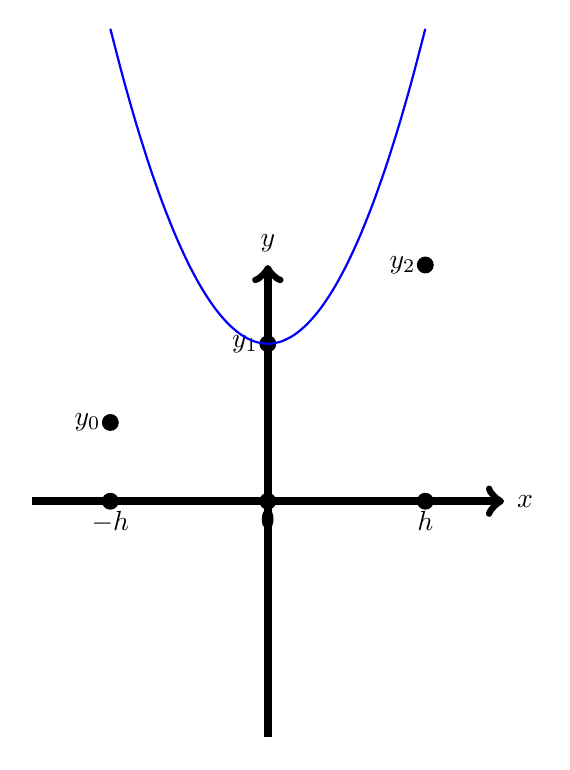
\begin{tikzpicture}
    % Koordinat eksenlerini çiz
    \draw[line width=1mm,->] (-3,0) -- (3,0) node[right] {$x$}; % x eksen
    \draw[line width=1mm,->] (0,-3) -- (0,3) node[above] {$y$}; % y eksen

    % x eksenindeki noktalar
    \draw[fill=black] (-2,0) circle (0.1) node[below] {$-h$};
    \draw[fill=black] (0,0) circle (0.1) node[below] {$0$};
    \draw[fill=black] (2,0) circle (0.1) node[below] {$h$};

    % y eksenindeki noktalar
    \draw[fill=black] (-2,1) circle (0.1) node[left] {$y_0$};
    \draw[fill=black] (0,2) circle (0.1) node[left] {$y_1$};
    \draw[fill=black] (2,3) circle (0.1) node[left] {$y_2$};

    % Parabolü çiz
    \draw[domain=-2:2, smooth, variable=\x, blue, thick] plot ({\x}, {\x*\x + 2});
\end{tikzpicture}
\end{center}

\section{Koordinat düzlemi üzerinde yer alacak h ve y değerleri belirlenir.}
$h = -h,0,h$\\
$y = y_{-1},y_{0},y_{1}$

\section{Polinomlar için x - h dönüşü yapılır.}
$x \leftrightarrow -h \longrightarrow c_{2}(-h)^2 + c_{1}(-h) + c_{0} $\\
$x \leftrightarrow 0 \longrightarrow c_{2}(0)^2 + c_{1}(0) + c_{0}$\\
$x \leftrightarrow h \longrightarrow c_{2}(h)^2 + c_{1}(h) + c_{0}$


\section{Katsayılardan oluşan sembolik matris oluşturulur.}
\begin{center}
$\begin{bmatrix}
h^2&-h&1&y_{-1}\\
0&0&1&y_{0}\\
h^2&h&1&y_{1}\\
\end{bmatrix} $ 
\end{center}

\section{İndirgenmiş eşelon matrisin hesaplanmasında kullanılacak algoritma belirlenir.}
Adım 1. m × n matrisi A ile başlayın. Eğer A = 0 ise, Adım 7'ye geçin.  \\
Adım 2. En sola yerleşmiş sıfır olmayan bir sütunu belirleyin. \\
Adım 3. Bu sütunun en üst pozisyonuna (bu pozisyonu pivot pozisyon olarak adlandırıyoruz) bir yerine getirmek için elementer satır işlemlerini kullanın.  \\
Adım 4. Pivot pozisyonun altına (kesinlikle) sıfır yerleştirmek için elementer satır işlemlerini kullanın.  \\
Adım 5. Pivot pozisyonunun altında (kesinlikle) sıfır olan başka satırlar yoksa, Adım 7'ye gidin.  \\
Adım 6. Pivot pozisyonunun altındaki satırlardan oluşan alt matrise Adım 2-5'i uygulayın.  \\
Adım 7. Elde edilen matris satır basamak formundadır.  \\
Daha fazla işlem yapmak için aşağıdaki adımları takip edebilirsiniz, Satır Basamak Formunu Azaltma  \\
Adım 8. Adım 7'de elde edilen satır basamak formundaki tüm öncül birleri belirleyin.  \\
Adım 9. Adım 8'deki öncül bir içeren en sağdaki sütunu belirleyin (bu sütunu pivot sütunu olarak adlandırıyoruz).  \\
Adım 10. Pivot sütunundaki öncül birin üzerindeki tüm sıfır olmayan girişleri silmek için tip III elementer satır işlemlerini kullanın.  \\
Adım 11. Pivot sütununun solunda başka öncül bir içeren sütun kalmadıysa, Adım 13'e gidin.  \\
Adım 12. Pivot sütunun solundaki sütunlardan oluşan alt matrise Adım 9-11'i uygulayın.  \\
Adım 13. Elde edilen matris azaltılmış satır basamak formundadır.  \\

\section{İndirgenmiş eşelon matrisin oluşturulması için katsayılardan oluşan başlangıç matrisi oluşturulur.}
\begin{center}
$\begin{bmatrix}
1&-1&1&y_{-1}\\
0&0&1&y_{0}\\
1&-1&1&y_{1}\\
\end{bmatrix} $ 
\end{center}

\section{Adım adım indirgenmiş matris hesaplanır.}
\begin{center}
$PivotRow= 0, Pivot: 0, (R3 \leftarrow R3 + R1 * -1) $\\
$\begin{bmatrix}
1&-1&1&y_{-1}\\
0&0&1&y_{0}\\
1&-1&1&y_{1}\\
\end{bmatrix} $ 
\end{center}

\section{İndirgenmiş eşelon matris}
\begin{center}
$\begin{bmatrix}
1&0&0&((y_{-1}) + ((y_{1} - (y_{-1})) * 0.5)) - y_{0}\\
0&1&0&(y_{1} - (y_{-1})) * 0.5\\
0&-0&1&y_{0}\\
\end{bmatrix} $ 
\end{center}


\end{document}